\documentclass[UTF8]{ctexart}
\usepackage{titlesec}
\usepackage{fancyhdr}
\usepackage{geometry}
\usepackage{graphicx}
\usepackage{caption}
\geometry{left=1.0in,right=1.0in,top=0.3in,bottom=0.3in}

\pagestyle{fancy}
\fancyhf{} 
\ctexset{
    section={
        format=\raggedright
    }
}

\begin{document}

\title{\vspace{0cm}第五次作业}
\author{程远2234412848}
\date{}
\maketitle

\section{如何获取网站IP地址}
在命令行中输入ping news.xjtu.edu.cn并运行,在查看网站延迟时即可
获取网站的IP地址。

\begin{figure}[h]
    \centering
    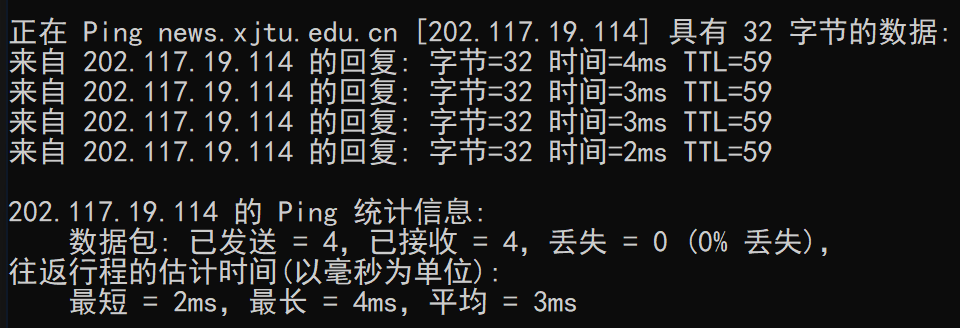
\includegraphics[width=1.0\textwidth]{res.png}
    \caption*{运行结果截图}
    \end{figure}
由图可知,该网站IP地址为202.117.19.114。

\section{如何从服务器获取zyxw.htm网页到客户端}
访问zyxw.htm网页后,浏览器会向DNS发送请求,要求返回该网站的IP地址。在浏览器获取到IP地址后,
它会通过TCP(Transmission Control Protocol)协议与服务器建立连接。在服务器收到连接请求后,
会向浏览器发送确认信息,如果信息有误,两者会重新尝试建立连接。连接建立后,浏览器向服务器发送
HTTP(Hypertext Transfer Protocol)请求,请求获取zysw.htm的内容。服务器收到请求后,即通过HTTP相应将页面的HTML内容发送到客户端。

\section{描述zyxw.htm的HTML界面}
HTML(Hypertext Markup Language)是一种标记语言,用于创建网页。它由各种元素组成,如标题、段落、链接、图像等,
这些元素描述了页面的结构、内容和样式。打开zyxw.htm后进行检查,部分页面如下。

\newpage

\begin{figure}[h]
    \centering
    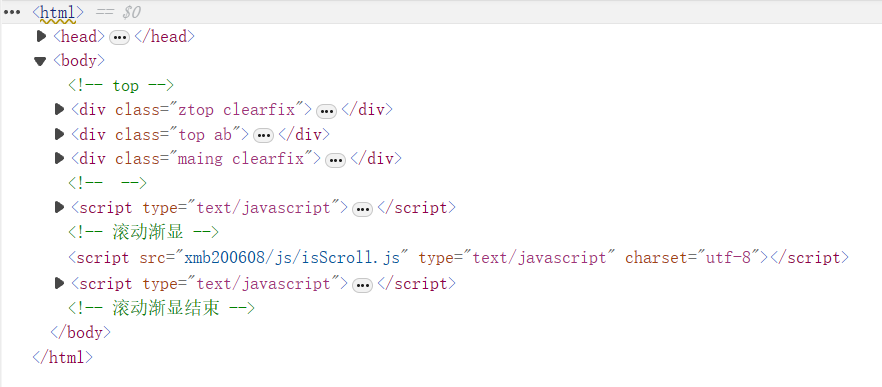
\includegraphics[width=1.0\textwidth]{demo1.png}
    \caption*{运行检查后的界面}
    \end{figure}

    在这个界面中,我们可以看到head和body两个部分,还可以看到用于指定utf-8的编码的语句。如果在body中继续探索,
    还可以找到描述西安交通大学logo出现动画的具体语句,如下。

\begin{figure}[h]
    \centering
    
\includegraphics[width=1.0\textwidth]{demo2.png}
    \caption*{logo出现动画语句}
    \end{figure}

可以看到,蓝色部分选中的“fadeInUp”字符串指定了logo出现时的动画,在这里具体向上淡入。
重新加载该网站,发现该logo确实为向上淡入出现,与HTML语句一致

\section{如何选择路径}
选择从计算即到网站服务器的路径包括以下步骤。当访问网站请求提出后,计算器发送一个HTTP请求到路由器或交换机。
下以路由器为例,当路由器收到请求后,会查看路由表,路由表中储存了目标IP地址与下一跳路由器的映射。
路由器通过路由表找到数据包发送的下一个路由器后,递归地进行这一过程。在这个递归过程中,路由器会
动态地确定最佳的传输路径,保证数据包能够高效地到达目标服务器。如果数据包需要通过局域网内部传输,
交换机会根据目标地址将数据包合理传输,找到下一个设备。最终,数据包通过多个路由器传输,抵达目标网站的服务器。
\end{document}